\documentclass{beamer}

%\usepackage[colorlinks=true, linkcolor=blue, urlcolor=blue, citecolor=blue]{hyperref}

% Set hyperref options using \hypersetup
\hypersetup{
  colorlinks=true, 
  linkcolor=blue, 
  urlcolor=blue, 
  citecolor=blue
}

\usepackage{verbatim}
\usepackage{listings}

\setbeamertemplate{footline}[frame number]

\lstset{
  basicstyle=\ttfamily,
  breaklines=true
}

\title{Project Management for Academia and Reproducible Science}
\author{Jeppe Søndergaard Johansen, SODAS Ph.D Fellow}
\date{\today}

\begin{document}

\begin{frame}
\titlepage % This will print the title, author, and date
\end{frame}

\begin{frame}{Table of Contents}
  \tableofcontents
\end{frame}

\section{Motivation}

\begin{frame}{Outline}
\begin{itemize}
    \item Most students have limited experience with big projects.
    \item Best practices consume very few resources – usually they consume less than bad practices.
    \item Science should be reproducible!
    \begin{itemize}
        \item \href{https://www.nature.com/articles/d41586-021-02211-4}{30\% genetics papers have Excel autocorrect errors.}
    \end{itemize}
\end{itemize}
\end{frame}


\begin{frame}{The ideal}

\begin{itemize}
    \item People getting access to your project should be able to push a single button and reproduce your results!
    \item The fewer steps an outsider needs to takes, the better.
    \item You should not feel anxious about running your project, and it should always give you the same answers!
    \item Cattle vs. Pets.
\end{itemize}

\end{frame}

\begin{frame}{My way into project management}
\begin{itemize}
    \item RA work.
    \item Software company.
    \item Worked in the Ministry of Education.
\end{itemize}
\end{frame}

\begin{frame}{Consideration}
\begin{itemize}
    \item Project structure
    \item Word Processor
    \item Reference manager
    \item Version control (and the elusive back-up)
    \item Data processing tools
    \item Project Operations (ProjOps)
\end{itemize}
\end{frame}

\begin{frame}{Cheat code! Cookie cutter}
\begin{itemize}
    \item Exercise (5 minutes)
    \item Easy way to begin – use my cookie-cutter project.
    \item \url{https://github.com/JakartaLaw/datascience-template}
    \begin{enumerate}
        \item Download Cookiecutter (following the instruction from the webpage): \url{https://cookiecutter.readthedocs.io/en/2.1.0/}
        \item Download the template and create a new project.
        \item Run: \textit{cookiecutter datascience-template}
        \item Run: \textit{make scaffold}
        \begin{itemize}
            \item If you are more interested in scaffolding I recommend the following tutorial: "How To With John Wilson" on HBO, Episode 2 "How to Put Up Scaffolding".
        \end{itemize}
    \end{enumerate}
\end{itemize}
    
\end{frame}

\section{Structuring and Writing a Project}

\begin{frame}{Scaffolding}
\begin{itemize}
    \item A project will usually have a structure along the lines: \begin{semiverbatim}
    
/data

/src

/output

/manuscript

Makefile

.gitignore

environment.yaml

README.md
\end{semiverbatim}   
\item Let's go through the individual files and folders.
\end{itemize}
 
\end{frame}

\begin{frame}{/data}

\begin{itemize}
    \item The data folder contains all the data used in the project.
    \item Usually, you will separate this into two folder: \textbf{processed} and \textbf{raw}.
    \item YOU CAN NEVER MANIPULATE YOUR RAW DATA. A GRAVE SIN!
    \item You keep your old datasets and do sequential manipulation.
    \begin{itemize}
        \item \textbf{RAW\_DATA.parquet} transformed to \textbf{clean\_data.parquet} transformed to \textbf{analysis\_data.parquet}.
        \item In general keep the temporary data sets.
    \end{itemize}
    \item Use open formats for data and preferably typed dataformats. .xlsx $<$ .CSV $<$  .parquet. Just use parquet if possible.
    \begin{itemize}
        \item Also, parquet works well with the library Polars, which is a big improvement coming from Pandas when manipulating data.
    \end{itemize}
\end{itemize}
    
\end{frame}

\begin{frame}{/src}
    \begin{itemize}
        \item You contain all your code (python, R, Stata etc.) files in this directory.
        \item Often you will have a sub-directory for files that do data. manipulations/data cleaning and a sub-directory for files that generate outputs, such as regression tables, summary statistics, and figures. In general, consider these to be separate entities:
        \begin{itemize}
            \item Files that produce data set.
            \item Files that produce output.
        \end{itemize}
        \item Finally, consider making a separate utility file that contains classes and functions for creating outputs. These should be easily configurable. Then you will have a single entry point for changing all you layouts of your manuscript!  
    \end{itemize}
\end{frame}

\begin{frame}{/output}
    \begin{itemize}
        \item You have usually two sub-folders in your output
        \begin{itemize}
            \item figures
            \item tables
        \end{itemize}
        \item If using LaTeX export your tables as .tex files. most regression libraries and Pandas allow for exporting as .tex files. Makes resizing of tables etc. much easier.
        \item Formats for figures can range from JPEG, PNG and PDF. LaTeX should have an easier time compiling PDF apparently, but not a big issue.
        \item Don't use screenshots for saving figures and tables. These should be exported as part of your code – again, remember running your project should automatically produce all the necessary outputs.
    \end{itemize}
\end{frame}

\begin{frame}{/manuscript}
    \begin{itemize}
        \item This is where all your files for your manuscript are located. You can use whatever format you desire, I would however recommend LaTeX –especially, after Chat GPT makes the boilerplate easy.
        \item LaTeX allows for compiling multiple documents together, so I would suggest a structure:
        \begin{semiverbatim}
    
/sections

main.tex
\end{semiverbatim}
    \item Where sections contain \textit{introduction.tex}, \textit{analysis.tex}, i.e. all the different parts of your manuscript. You can import them into your main.tex document using the command \textbf{input}
    \item You can consider having a style sheet for your main document in LaTeX as well.
    \end{itemize}
\end{frame}

\begin{frame}{Other files}
    \begin{itemize}
        \item .gitignore: Is for all the files, that should not be checked into git. Git will be discussed later.
        \item environment.yaml: Is for creating your python environment. Usually, you will have a conda environment with specific packages etc. save the specifications to environment.yaml file, so other people can create your exact environment. This will be discussed later.
        \item README.md: Is for new comers (and sometimes yourself) to understand the ins and outs of your project. Basically, documentation.
        \item Makefile: Is the single entry point used for running your project! This is the metaphoric \textit{one push button}, that can run everything. This will be discussed later.
    \end{itemize}
    
\end{frame}


\section{Word Processors}
\begin{frame}{Which formats}
\begin{itemize}
    \item Word / Google Docs
    \begin{itemize}
        \item Pro: Low barrier of entry. Google Docs allow for collaboration. \item Cons: Hard to integrate into a highly automated workflow. Does not work well with Git. Very fragile!
    \end{itemize}
    \item LaTeX (Recommended)
    \begin{itemize}
        \item Pro: Works very well for collaboration. Overleaf and Live Share in VS Code. Integrates very well into an automatic workflow. Mature ecosystem.
        \item Cons: Steep learning curve. Lots of boilerplate. Less of a problem after the introduction of Chat GPT.
    \end{itemize}
    \item Markdown or Quarto MD
    \begin{itemize}
        \item Pro: Works very well for collaboration. Overleaf and Telemetry in VS Code. Integrates very well into an automatic workflow.
        \item Uses LaTeX as a backend for compilation and can be hard to customize. The ecosystem is changing a lot. Have not yet have a good experience with Quarto!
    \end{itemize}
\end{itemize}
    
\end{frame}

\begin{frame}{More on LaTeX}

\begin{itemize}
    \item Is not a WYSIWYG format like word or Google Docs.
    \item Instead you have a mark up language, which you compile into final documents.
    \item You separate styling into a preamble (i.e. before your document typing begins).
    \item Very popular in quantitative sciences due to its good math typesetting.
    \item You can separate your manuscript into smaller files, which you then can compile into a single big one! Makes rearranging, "out commenting" and multiple versions of different sections easier.
    \item Exercise (10 minutes):
        \begin{itemize}
            \item Login to overleaf.com (maybe you need to make a profile).
            \item Use Chat GPT to generate an example document with LaTeX and let it explain the different parts of it. Especially consider:
            \begin{itemize}
                \item What is the difference between the preamble and the document. How to separate your manuscript into smaller pieces. How to import figures and tables.
            \end{itemize}
            \item Try to compile the code!
        \end{itemize}
\end{itemize}
\end{frame}

\begin{frame}{Writing LaTeX}
\begin{itemize}
    \item Two candidates:
    \begin{itemize}
        \item VS Code
        \begin{itemize}
            \item Use the LaTeX VS code extension.
            \item You can collaborate using Git. Needed anyway.
            \item Using Live Share.
            \item An interesting alternative is the Visual Studio workspace option – however, I have no experience with this.
        \end{itemize}
        \item Overleaf (Recommended)
            \begin{itemize}
                \item Browser based (think like Google Docs for Overleaf).
                \item Works very well with Zotero and Git+Github.
                \item Use Grammarly for better spell check. Apparently a new LLM tool for spell check also exists (no experience).
            \end{itemize}
    \end{itemize}
\end{itemize}
\end{frame}

\section{Version Control, Backup and Collaboration}

\begin{frame}{Git and Github}
\begin{itemize}
    \item How should you collaborate on a project?
    \item You need to be able to integrate multiple peoples' work.
    \item You need also to do version control. i.e. you make a change to your manuscript, but you want to keep the old version as well? It cannot be optimal to have 10 documents named \textit{main\_v1, main\_v2,} ...
    \item You can send things over Facebook messenger? You could use dropbox?
    \item better idea, use Git for version control and use Github for collaboration.
    \item You have a .gitignore file, which stores which files NOT to track.
\end{itemize}
\end{frame}

\begin{frame}{Git basics}
    \begin{itemize}
        \item You check in files. Git keeps a log of the changes of the individual files.
        \item You \textit{commit} changes. You can also revert them (in contrast with Dropbox).
        \item You can \textit{branch} out your project. Your project becomes a tree, not a one-way road.
        \item You write messages when you commit, so you have a log of your document and how it evolved. Good commit messages allow you for rediscover why you did what you dit.
    \end{itemize}
\end{frame}

\begin{frame}{Git tree}
    \begin{figure}
        \centering
        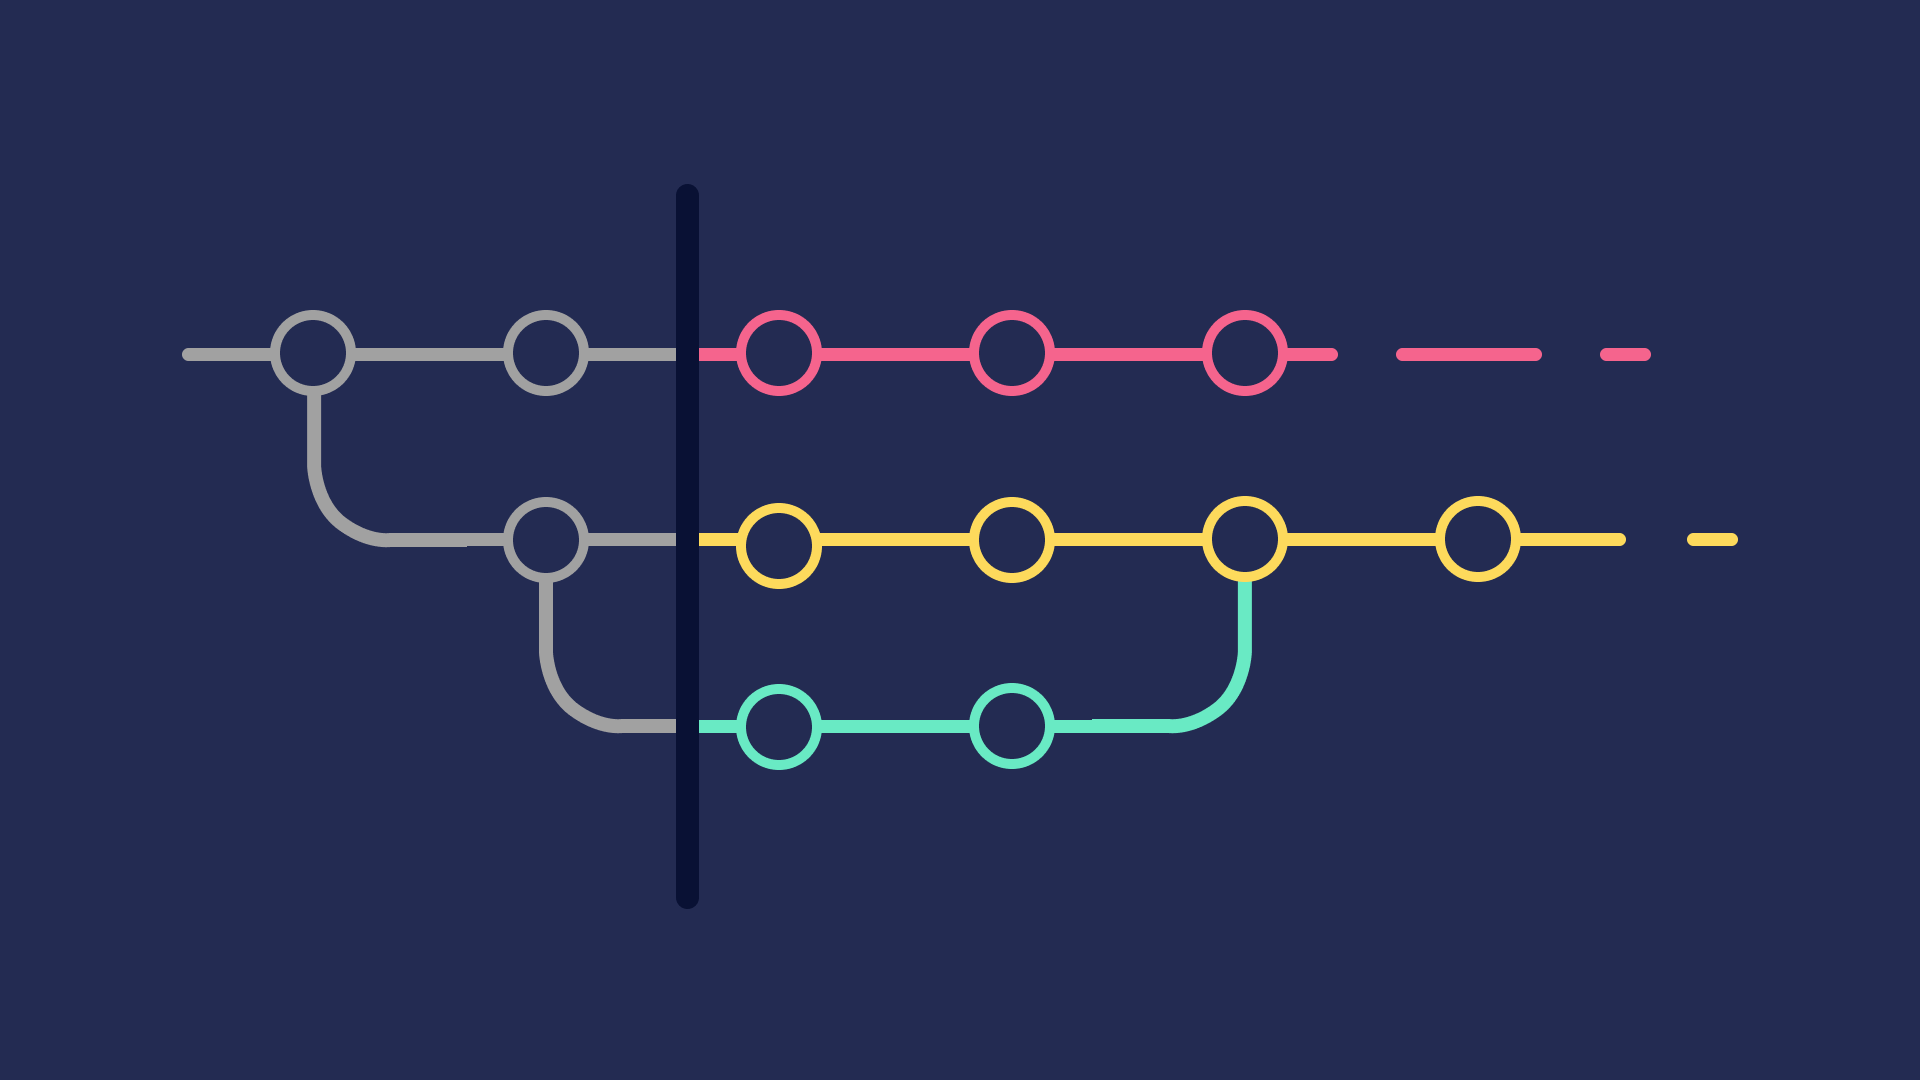
\includegraphics[width=0.8\textwidth]{slides/improved-git-flow-2.png}
        \caption{Git tree illustration}
        \label{fig:enter-label}
    \end{figure}
\end{frame}

\begin{frame}{Github basics}
    \begin{itemize}
        \item The Dropbox equivalent for Git.
        \item An online hub for your Git repositories (folders tracked by Git).
        \item This is the easiest way to share your work with the world in general and between collaborators. You can have both private and public repositories.
        \item Traditionally you used Git from the terminal, but with VS Code and Github desktop, that makes it easier.
        \item Exercise (10 minutes)
        \begin{itemize}
            \item Make a Github account.
            \item Download Github Desktop.
            \item Use Chat GPT to ask about how to use Git and Github. Especially, investigate the key concepts such as:
            \begin{itemize}
                \item Repository, Commit, Branch, Clone, Remote, Fetch, Pull, Push, Merge, Stash, Conflict, Checkout, Fork, Pull Request 
            \end{itemize}
            \item Pro tip: Have a nice Github profile – recruiters look at it! Have a cool project!
        \end{itemize}
    \end{itemize}
\end{frame}


\section{Data processing tools}

\begin{frame}{Data Processing with Python}

\begin{itemize}
    \item You already know how to use Python here are some extra tips and tricks.
    \item Notebooks are easy to use – however consider using standard .py files and install the Python extension to VS code. You can make cells writing $\#\%\%$ and do interactive programming. Notebooks are bad for sequential execution of files and version control!
    \item Use Parquet when saving files. Most empirical work is data cleaning. Polars is a nice alternative to Pandas. Try it out.
    \item You can load YAML files into python easily (becomes a dictionary). This can be a nice way to centralize the configuration of your project.
\end{itemize}
\end{frame}

\begin{frame}
    \begin{itemize}
    \item Separation of concerns. Most data projects are sequential (as oppose to other software), first you clean data, then you do descriptive statistics and analysis. This should go into different files. You have a single file that executes them all (Makefile).
    \item You might want to consider R when doing certain analytics work. Still have a better ecosystem for statistics.
    \item Use Conda (recommended) or Pipenv or Poetry for your python environment. Save your environment into a file so outsiders can recreate it (environment.yaml).
    \end{itemize}
\end{frame}

\section{Project Operations (ProjOps)}

\begin{frame}{Project Operations}
\begin{itemize}
    \item An analog to DevOps.
    Why?
    \item There is a suite of tools (as presented) you use for data science projects.
    \item We have talked about these, but how do we combine them? The answer: Makefiles
    \item Is a platform-agnostic tool for executing files say Python, LaTeX and R.
\end{itemize}
\end{frame}

\begin{frame}
  \frametitle{What is \texttt{make}?}
  \begin{itemize}
    \item A build automation tool.
    \item Used to automatically build and manage dependencies.
    \item Operates on a file called a \texttt{Makefile}.
    \item Commonly used in software projects that use C and C++, but also nice for data science projects.
  \end{itemize}
\end{frame}

\begin{frame}[fragile]
  \frametitle{Basic Structure of a Makefile}
  \begin{lstlisting}
target: dependencies
	commands
  \end{lstlisting}
  \begin{itemize}
    \item \texttt{target} is the name of the file to be generated.
    \item \texttt{dependencies} are files that \texttt{target} depends on.
    \item \texttt{commands} are the shell commands that produce the \texttt{target}.
    \item The make system considers whether or not the the file dependencies have been updated since the file changed, so it only runs the necessary stuff.
  \end{itemize}
\end{frame}

\begin{frame}
  \frametitle{Why Use \texttt{make}?}
  \begin{itemize}
    \item Automatically manages project builds.
    \item Ensures that only necessary parts are rebuilt.
    \item Makes it easy to manage large projects.
    \item Aids in reproducibility.
    \item Use Chat GPT for creating them. Also VS Code has a nice extension that helps with the syntax!
  \end{itemize}
\end{frame}

\section{Reference Tool and Literature Review}

\begin{frame}{Reference Tool}

\begin{itemize}
    \item There are multiple options, but I feel most people have settled on \textbf{Zotero}. Also what I will talk about.
    \item Makes it possible to centralize all your papers.
    \item Have a nice Chrome extension, to save papers and information.
    \item Exports .bib files for references.
    \item You can have an online user for Zotero, and through there connect your Zotero account to Overleaf.
    \item Consider the Zotero extension \textit{Better Bibtex} for better bib-files. Especially, automatic bib file updating!
    \begin{itemize}
        \item A nice opensource project one of you should built is an VS Code extension that integrates Zotero Web for automatic bib-files in VS Code. Probably could be done in a day or two! 
    \end{itemize}
    \item Zotero allows for saving and reading the actual paper. All your PDFs in one place!
\end{itemize}
    
\end{frame}

\begin{frame}{Literature Review}
\begin{itemize}
    \item Your thesis work usually start by formulating a tentative research question: \textit{"How are women impacted differently than men by automation software?"}
    \item Before studying this more closely and narrowing in the RQ, you need to have an overview of the existing literature.
    \item How can you effectively go about this process?
    \item The stages of a literature review (numbers can very a lot):
    \begin{enumerate}
        \item Formulate RQ
        \item Reading review articles
        \item Narrow relevant articles for abstract readings ($\approx$ 200+ articles)
        \item Isolate pre-manuscript articles ($\approx$ 50 - 100 articles)
        \item Find articles that actually go into your finished manuscript ($\approx$ 20 - 30 articles).
        \item In general you will find 1 to 3 key articles that you draw very heavily on.
        \item You will probably begin to look at cites from the key articles as well.
    \end{enumerate}

\end{itemize}    
\end{frame}

\begin{frame}{Getting a long list of abstracts}
\begin{itemize}
    \item The 3 most common databases are Google Scholar, Scopus and Web of Science. I would suggest using WOS.
    \item Use wildcard symbols (astrix, boolean operators etx). WOS is good for this. Adjust you search query until you have a manageable number of articles.
    \item Consider thinking in either PICO or PEO:
    \begin{itemize}
        \item PICO (Population, Intervention, Comparison, Outcome). Great for quantitative stuff.
        \item PEO  (Population, Exposure, Outcome). Great for qualitiative.
    \end{itemize}
    \item Since you are at UCPH you can use \textbf{kb.dk} to get extra access to certain articles.
    \item \url{Elicit.org} is a new tool that might also be night too play around with for finding articles.
    \item WOS allows you to export your search results (author, source, abstract) into a single file. Use this to read the abstracts and narrow down the relevant articles.
\end{itemize}
\end{frame}

\begin{frame}{Zotero + Literature review}
\begin{itemize}
    \item Exercise (15+ minutes)
    \begin{enumerate}
        \item Download Zotero and make an online profile. Also get the Zotero Chrome plugin: Zotero connector
        \item Make public collection on Zotero Web and integrate it with your Zotero web.
        \item Find a random article on Arxiv and use Zotero connector to save the paper. Ensure it saves the metadata and the file to your computer. Update the bibfile on Overleaf, ensure the bibfile looks correct. Finally use Chat GPT to add the reference into your manuscript!
        \item Go to WOS and make a search query. Adjust til you are in the ballpark of 50 articles.
        \item Export the search results (Author, source, abstract) and download it.
        \item just quickly google the tools: scite.ai, researchrabbit.ai and connectedpapers.com
    \end{enumerate}
    \item Look at \url{https://github.com/JakartaLaw/SODAS-project-management-reproducible-science/tree/main} for an example project
\end{itemize}
    
\end{frame}



\end{document}